\documentclass{standalone}
\usepackage{tikz}
\usepackage{ctex,siunitx}
\usepackage{tkz-euclide}
\usepackage{amsmath}
\usetikzlibrary{patterns, calc}
\usetikzlibrary {decorations.pathmorphing, decorations.pathreplacing, decorations.shapes,}
\begin{document}
\small
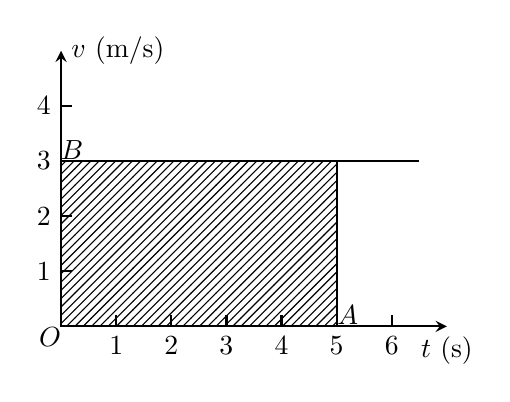
\begin{tikzpicture}[>=stealth, thick,scale=0.7]
  \draw [<->](0,5)node[right]{$v$ (\unit{m/s})}--(0,0)--(7,0)node[below]{$t$ (\unit{s})};
  \draw (5,3)--(5,0);
  \foreach \x in {1,2,3,...,6}
  {
      \draw(\x, 0) node[below]{$\x$} --(\x, .2);
  }
  \draw (0,3)--(6.5,3);
  \node at (.2,3.2){$B$};  \node at (5.2,0.2){$A$};  
  \foreach \y in {1,2,3,4}
  {
      \draw(0,\y)node[left]{$\y$}--(.2, \y);
  }
  \node at (-.2,-.2){$O$};
  \fill [pattern = north east lines] (0,0) rectangle (5,3);
\end{tikzpicture}
\end{document}